\subsection{Electromagnetic Calorimeter}
\label{ild:sec:ECAL}
%\writer{Jean Claude Brient, Wataru Ootani}{3}
The technological status of both the silicon based and the scintillator based option considered for the highly granular multi-layer sampling electromagnetic calorimeter is described in this secion. 

\subsubsection{Silicon option (SiECAL)}

In the past five years the developments of the silicon option of the electromagnetic calorimeter has mostly focused on the design and construction of technological prototypes of the detector, and on performing beam tests. 

So far square wafers with thicknesses between $325\,\upmu m$ and $650\,\upmu m$ processed from 6" silicon ingots have been used. 
An increased thickness of $725\,\upmu m$, already available from 6" ingots, would be conducive in case wafers from 8" ingots can be reliably produced. It would allow to reduce the number of ECAL layers to 26, without significant degradation of the energy resolution compared to the current baseline design of 30 layers (section~\ref{ref:subsec:subdetectors}). For the final detector, the ongoing technological developments allow to foresee to use diode matrices with a standard thickness of $725\,\upmu m$ produced from 20\,cm wafers, but the final choice of the ingot size will depend on the silicon producers chosen at the time of building the calorimeter.

% {\it COMMENT R.P.:  Altough 8" may have advantages over 6" it is as of today from my point of view by no means clear/sure that 8" is the option of choice. CMS HGCAL has chosen indeed 8" but there is no experience with mass production. This we may have in about two years from now. Note that the CMS Tracker stays with 6".}} 
% {\color{blue} The current technological developments have led to choosing 20\,cm wafers for making the diode matrices, with a standard thickness of up to 725 micrometers.}  

%When applied to ILD this would result in a slightly thicker electromagnetic calorimeter than foreseen in the baseline design.  It allows for reducing the number of layers from 30 to 26 (see section 5.1.2). without important  degradation of the electromagnetic energy resolution.

Fully integrated layouts of the silicon active sensor units (ASU) have been designed with the required dimension of $18 \times 18\,{\rm cm^2}$ comprising 1024 channels. One ASU hosts 16 SKIROC ASICs~\cite{Callier:2011zz,Suehara:2018mqk} to process 64 channels each. The top part of Figure~\ref{fig:det:SiWECAL_proto} shows two recent versions of the ASU, both assembled with standard ball grid array (BGA) packaging of the ASICs. 
The most recent version (\#13) features a separation between the power supply of the preamplifier and other power lines of the SKIROC ASIC. 
Big capacitances are integrated into the board design to avoid large current peaks during power pulsing. 
%Additionally for FEV13 the size of the adapter card that transmits the signals between the interface card for the digital readout and that carries the regulators for the power supply has been reduced. 
This as well as earlier versions of the ASU have been operated in power pulsed mode since 2013. The bottom part of Figure~\ref{fig:det:SiWECAL_proto} shows the mechanical housing that can hold up to ten ASUs used in beam tests at CERN and DESY since 2012~\cite{Boudry:2014bxa,Poeschl:2015jma}. 
%In 2018 a combined beam test with the SDHCAL technological prototype (see next section) has been carried out.

\begin{figure}[t!]
\centering
%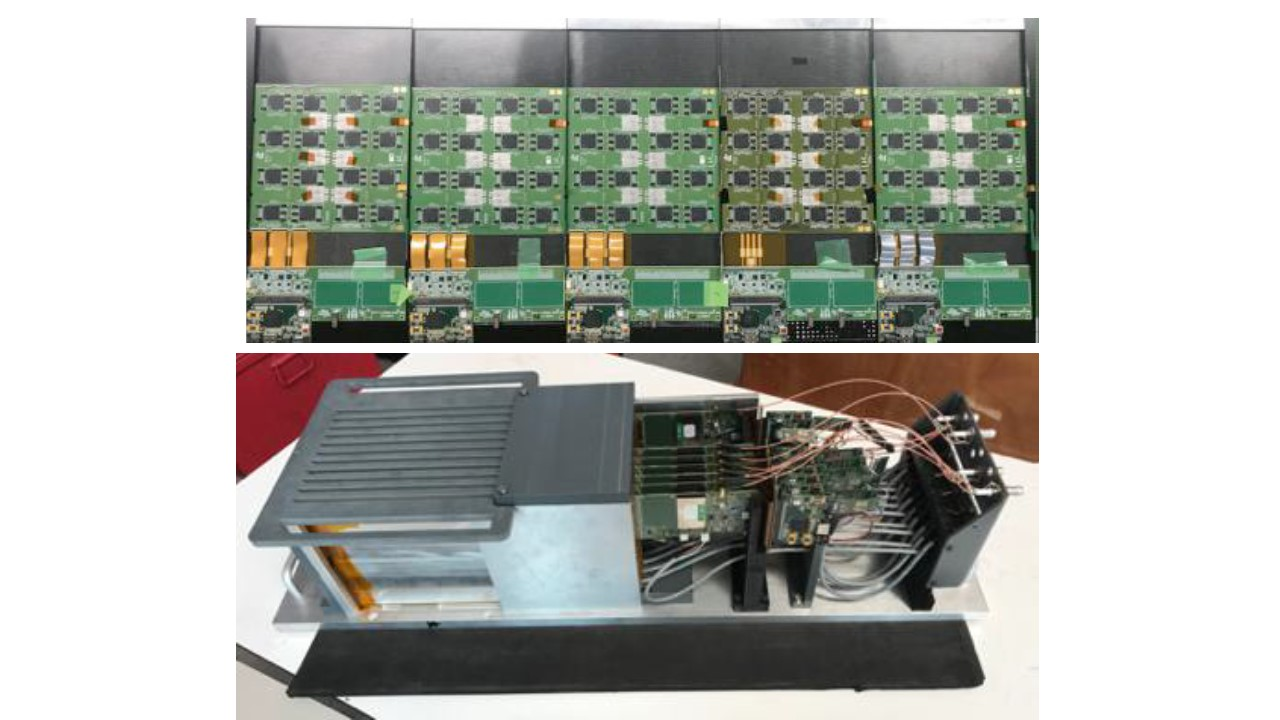
\includegraphics[width=1.0\hsize]{Detector/fig/SiWECAL_proto.jpg}
\begin{subfigure}{0.45\textwidth}
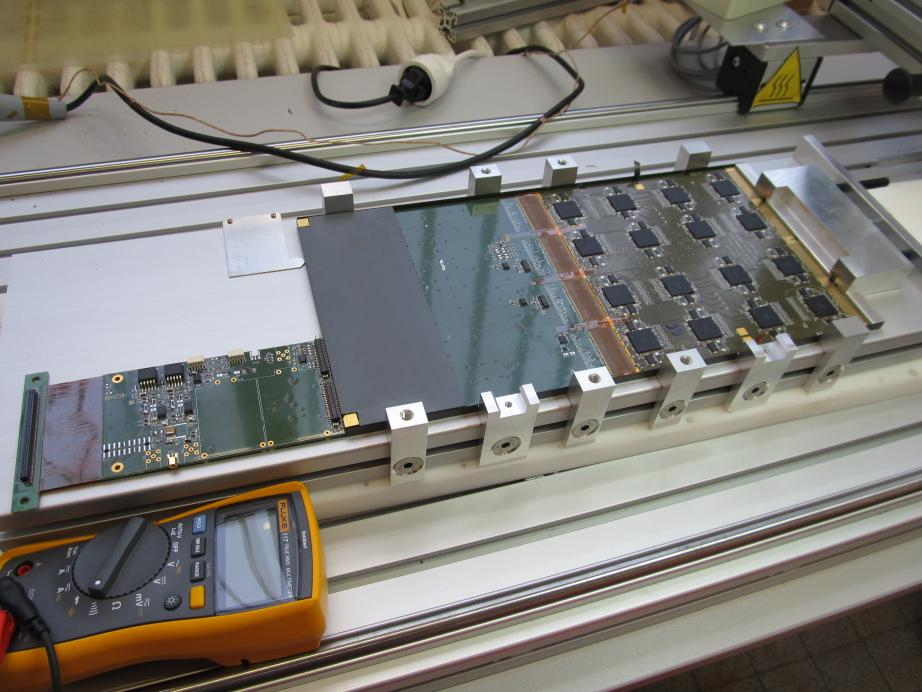
\includegraphics[width=0.9\hsize]{Detector/fig/siwecal-fev12.jpg}
\end{subfigure}
\begin{subfigure}{0.45\textwidth}
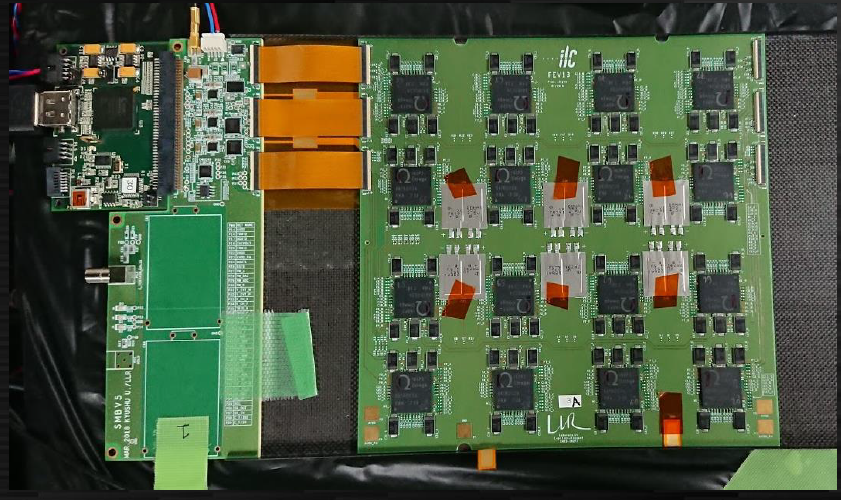
\includegraphics[width=1.1\hsize]{Detector/fig/siwecal-fev13.png}
\end{subfigure} \\ 
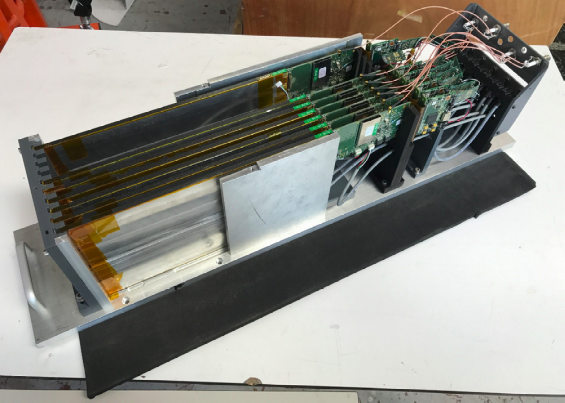
\includegraphics[width=0.50\hsize]{Detector/fig/siwecal-tp.png}
\caption{Technological prototype of the SiECAL. Top: integrated ASUs (left: version \#11, right: version \#13); bottom: mechanical housing with integrated layers of the SiECAL prototype used in beam tests at DESY and CERN.}
\label{fig:det:SiWECAL_proto}
\end{figure}



%\begin{figure}[t!]
%\centering
%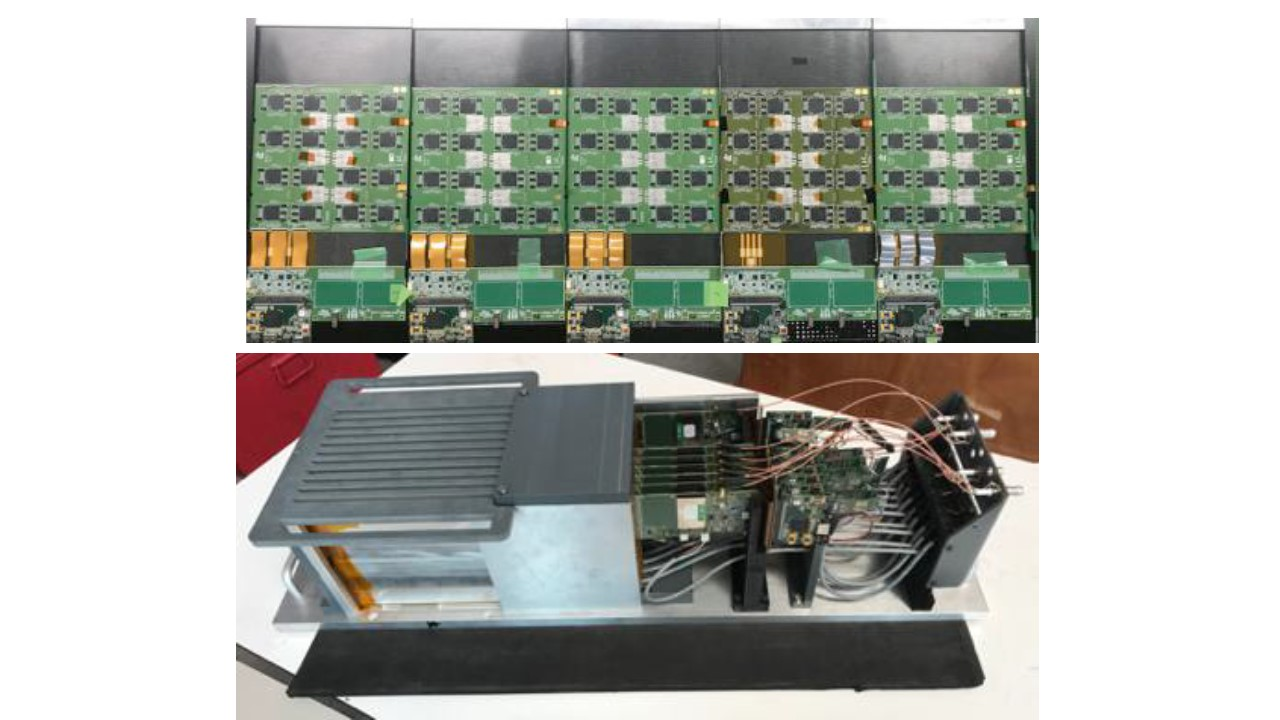
\includegraphics[width=1.0\hsize]{Detector/fig/SiWECAL_proto.jpg}
%\caption{Technological prototype of the SiECAL. Top: set of integrated sensor\&readout boards; bottom: 10-layers calorimeter prototype used in beam tests at DESY and CERN.}
%\label{fig:det:SiWECAL_proto}
%\end{figure}

The response of the SiECAL technological prototype to particles is as expected~\cite{Kawagoe:2019dzh}. The signal-over-noise ratio relevant for the internal ASIC trigger has been evaluated to be about 12.8 for a wafer thickness of $325\,\upmu m$. This value allows for setting the trigger threshold below the single MIP level with high efficiency. %although new dedicated beam tests are required to know the uncertainty and spread of this value among different modules and ASICs. 
The signal-over-noise at the level of charge measurement for triggered channels is 20.4 (Figure~\ref{fig:det:SiWECAL_signals} left), or better, depending on the wafer thickness. Therefore a threshold cut in the ASIC at 0.5 MIP can be applied without noise problems and with good efficiency.
%This ensures that all channels with a trigger just above noise level can be used in particle flow energy reconstruction.
 Response to high energy electrons has been measured at CERN in 2018 in a combined test with the SDHCAL (next section) as shown in Figure~\ref{fig:det:SiWECAL_signals} right.


%{\color{blue} A signal-to-noise ratio of 20 is measured for MIPs in single pads (Figure~\ref{fig:det:SiWECAL_signals} left). Such a large signal/noise ratio of MIPs is important for isolated particle identification in particle flow energy reconstruction. 
%Fi%rst response to high energy electrons has recently been measured at CERN in a combined test with the SDHCAL (Figure~\ref{fig:det:SiWECAL_signals} right). 
%The beam tests have also been used to validate the power pulsing of the front-end electronics required to minimise heat production within the calorimeter.
 %A new version of the detector slabs is currently in production from a joint development in LLR and Kyushu. A total number of 20 detection layers could be reached in the coming year.
% This will allow the construction of a full ECAL prototype to be used in test beams for measurements of the energy resolution.}

\begin{figure}[t!]
\centering
\begin{subfigure}{0.48\textwidth}
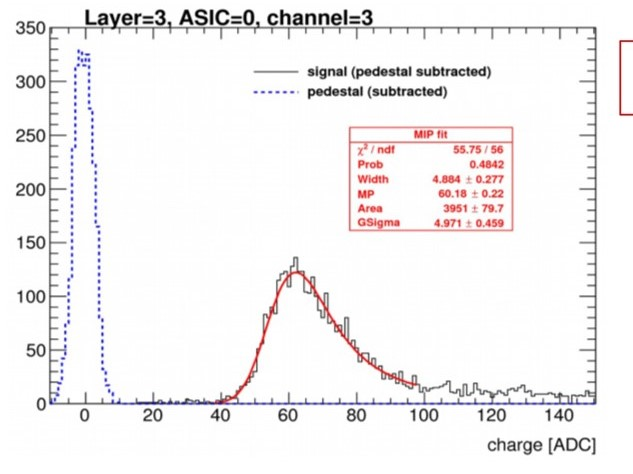
\includegraphics[width=1.0\hsize]{Detector/fig/SiWECAL_signals_layer.jpg}
\caption{}
\end{subfigure}
\begin{subfigure}{0.48\textwidth}
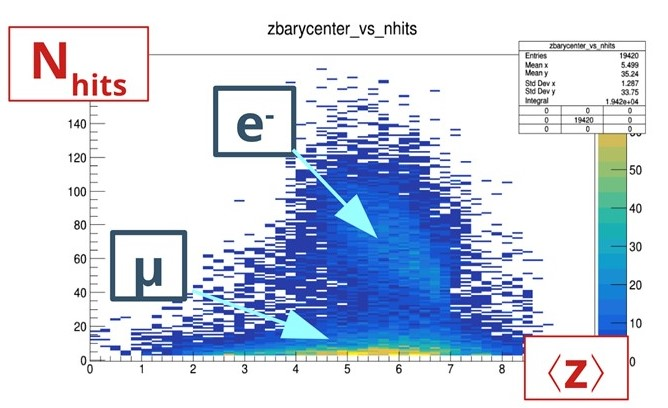
\includegraphics[width=1.0\hsize]{Detector/fig/SiWECAL_signals_energy.jpg}
\caption{}
\end{subfigure}
\caption{Particle response of the SiECAL prototype: (a) MIP response of a single pad. (b) Shower profile (number of pad hits as a function of longitudinal layer number) of muons and 80 GeV electrons.}
\label{fig:det:SiWECAL_signals}
\end{figure}

%{\color{blue} More developments are ongoing to reach the requirements of the full-size ILD detector. The layout of the sensitive layer diode matrices has been revisited since the technological prototype construction.}

%{\color{blue} A large detector slab with dimensions similar to those of the calorimeter modules has been built and tested with MIPs~\cite{Balagura:2017vvf} (Figure~\ref{fig:det:SiWECAL_dev} right).} 

A long detector slab featuring a chain of eight ASUs has been built (Figure~\ref{fig:det:siw-longslab}) and tested with MIPs~\cite{Magniette:2019nyg}. 
A 10\% signal drop has been observed along the full length of the slab and could be attributed to power voltage drops and clock reflections. An improved long slab is under construction to correct these effects and validate the system. 

\begin{figure}[t!]
\centering
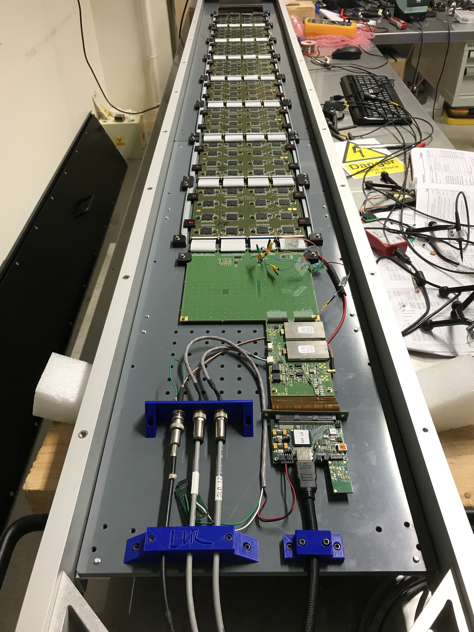
\includegraphics[width=0.32\hsize,angle=90]{Detector/fig/siwecal-longslab.png}
\caption{The first prototype of a long slab of the SiECAL.}
\label{fig:det:siw-longslab}
\end{figure}


 A new slab interface board for the digital readout of the ASUs, located at the end of the slabs, has been developed to meet the ILD integration constraints (Figure~\ref{fig:det:SiWECAL_slcards} left). The board integrates the digital readout of the SiECAL layers and hosts the regulators for the power supply of the ASUs,
 With a lateral size of about $4\times 18\,{\rm cm^2}$, this board already meets the tight space requirements of ILD. The board has been successfully used in a beam test in summer 2019 at DESY~\cite{bib:talk-twepp-jj}.
 The slab interface boards are connected via a flat control and readout kapton cable to a concentrator unit as illustrated in the right part of Figure~\ref{fig:det:SiWECAL_slcards}. 
 The distinguished feature of this solution is that the kapton cable can be guided along the sides of an alveolar structure hence avoiding bulky cabling. 
 
An ultra-thin ASU with an overall thickness of 1.2\,mm has also been developed. In this version the ASICs are mounted in recessed cavities of the PCB in a so-called chip on board (COB) packaging (Figure~\ref{fig:det:SiWECAL_cob}). 
 First tests of the COB ASUs have been successfully performed at the 2019 beam test at DESY~\cite{bib:talk-twepp-jj}. Clean MIP spectra have been recorded and the noise level is competitive with that of the BGA based ASUs built up to now. This is remarkable since the design of the board leaves relatively little room for decoupling capacitors. The flatness of this card  meets the specifications, but the yield has to be studied with industry. Further tests will be performed and industrial aspects will  have to be investigated further.
  % allowed for wafer gluing with a robot as for the other cards introduced above. 
%  Provided industrial aspects are under control, the FEV\_COB couild  allow for meeting the space constraints given in Fig.~\ref{fig:det:ECAL_readout}. 


% {\color{blue} A lot of R\&D is foreseen in the years coming essentially centred on the signal/noise ratio, the coherent noise, the fraction of dead pixels, and specific to our detector, a level of internal retriggering not manageable at ILC with the current version of the VFE ASIC.} 

The R\&D in the coming years will further emphasise system and integration aspects based on the current achievements. The planned R\&D includes a new version of the  ASIC with full zero suppressed readout, which implies an utmost stable pedestal level.

%\begin{figure}[t!]
%\centering
%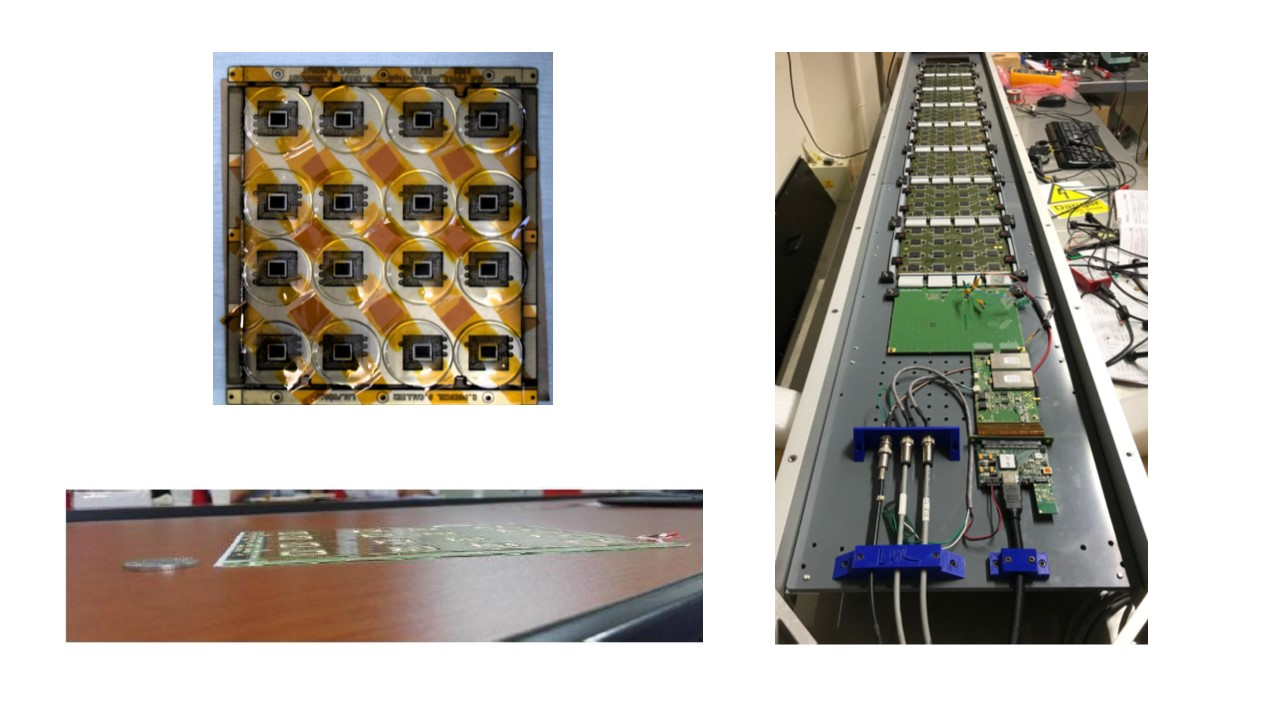
\includegraphics[width=1.0\hsize]{Detector/fig/SiWECAL_dev.jpg}
%\caption{SiECAL developments towards the final detector: thin chip-on-board sensors (left) and long slabs corresponding to ILD dimensions (right).}
%\label{fig:det:SiWECAL_dev}
%\end{figure}

\begin{figure}[t!]
\centering
\begin{subfigure}{0.48\textwidth}
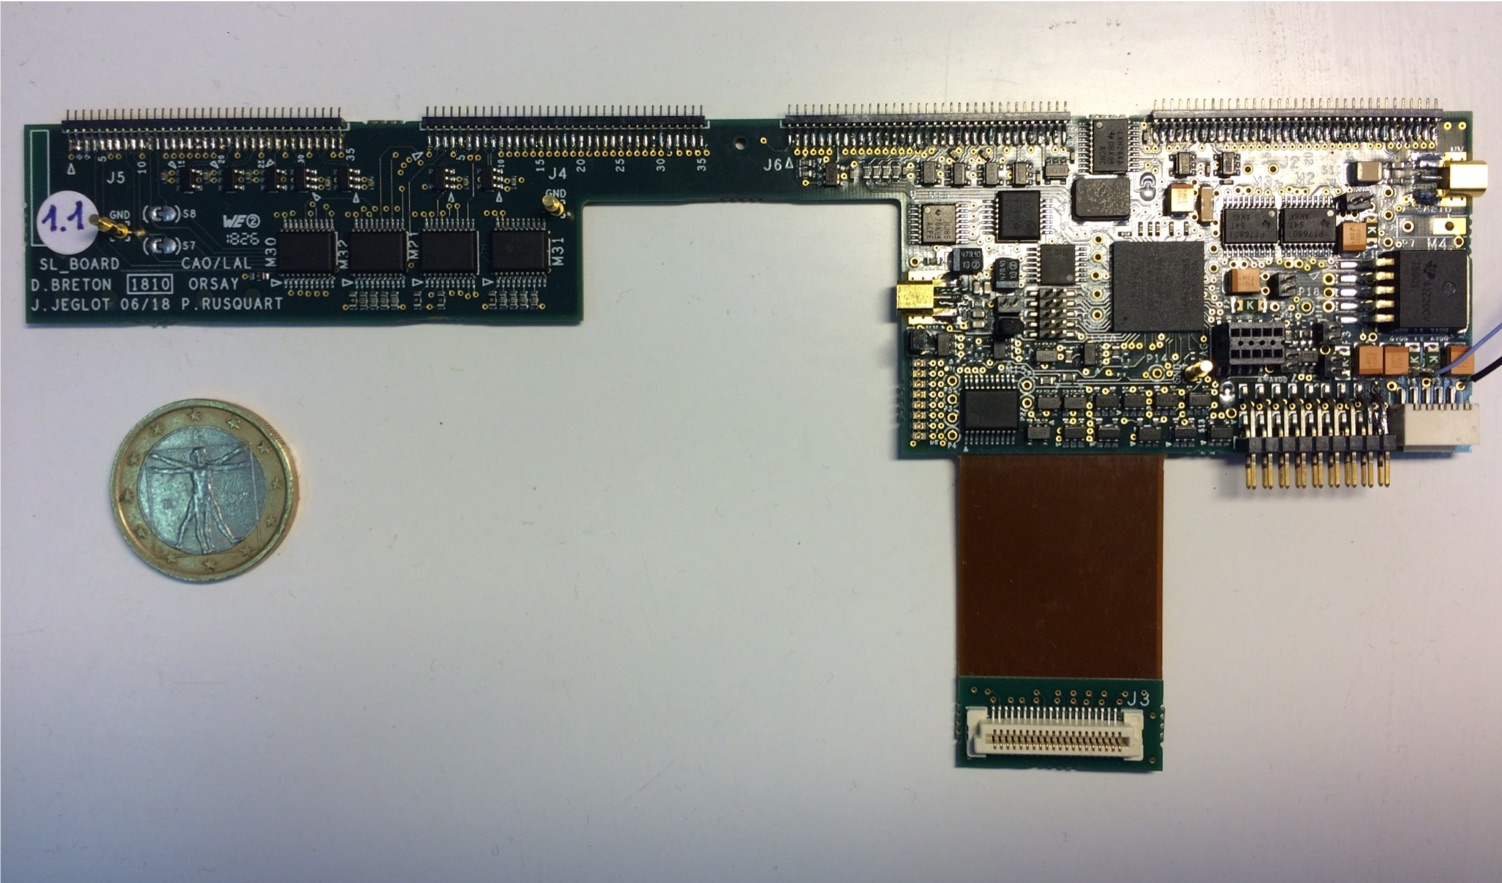
\includegraphics[width=1\hsize]{Detector/fig/siwecal-slboard.jpg}
\caption{}
\end{subfigure}
\begin{subfigure}{0.48\textwidth}
%\includegraphics[width=1.0\hsize]{Detector/fig/core-kapton.png}
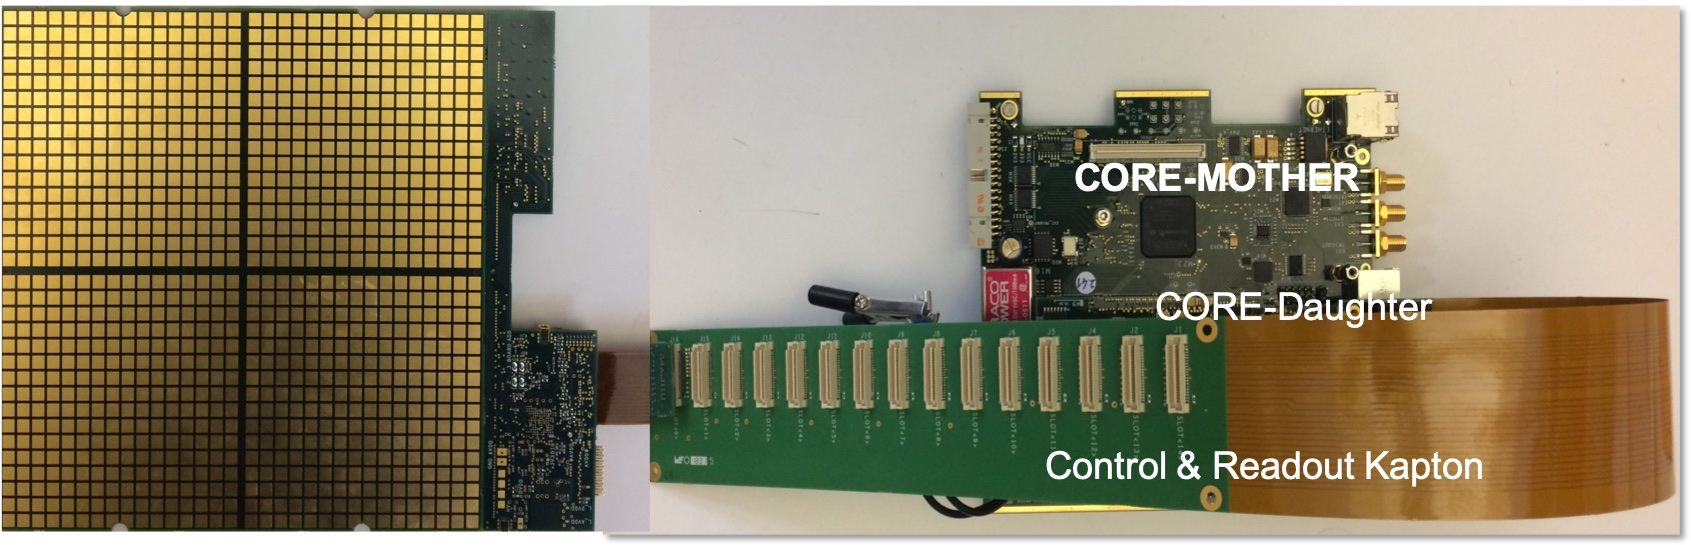
\includegraphics[width=1\hsize]{Detector/fig/siwecal-fevslcore.jpg}
\caption{}
\end{subfigure}
\caption{(a) Slab interface board for the digital readout and the power supply of the SiECAL layers. (b) Ensemble of one ASU with its slab interface board, control and readout kapton, and concentrator unit.}
\label{fig:det:SiWECAL_slcards}
\end{figure}


\begin{figure}[t!]
\centering
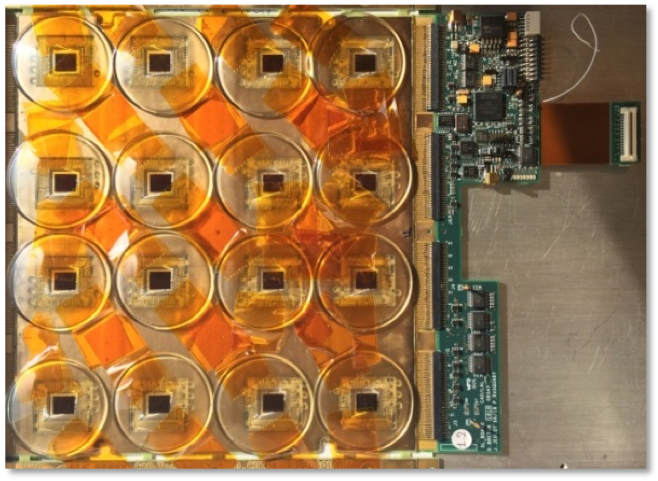
\includegraphics[width=0.35\hsize]{Detector/fig/siwecal-cob-sl.png}
%\includegraphics[width=1.0\hsize]{Detector/fig/core-kapton.png}
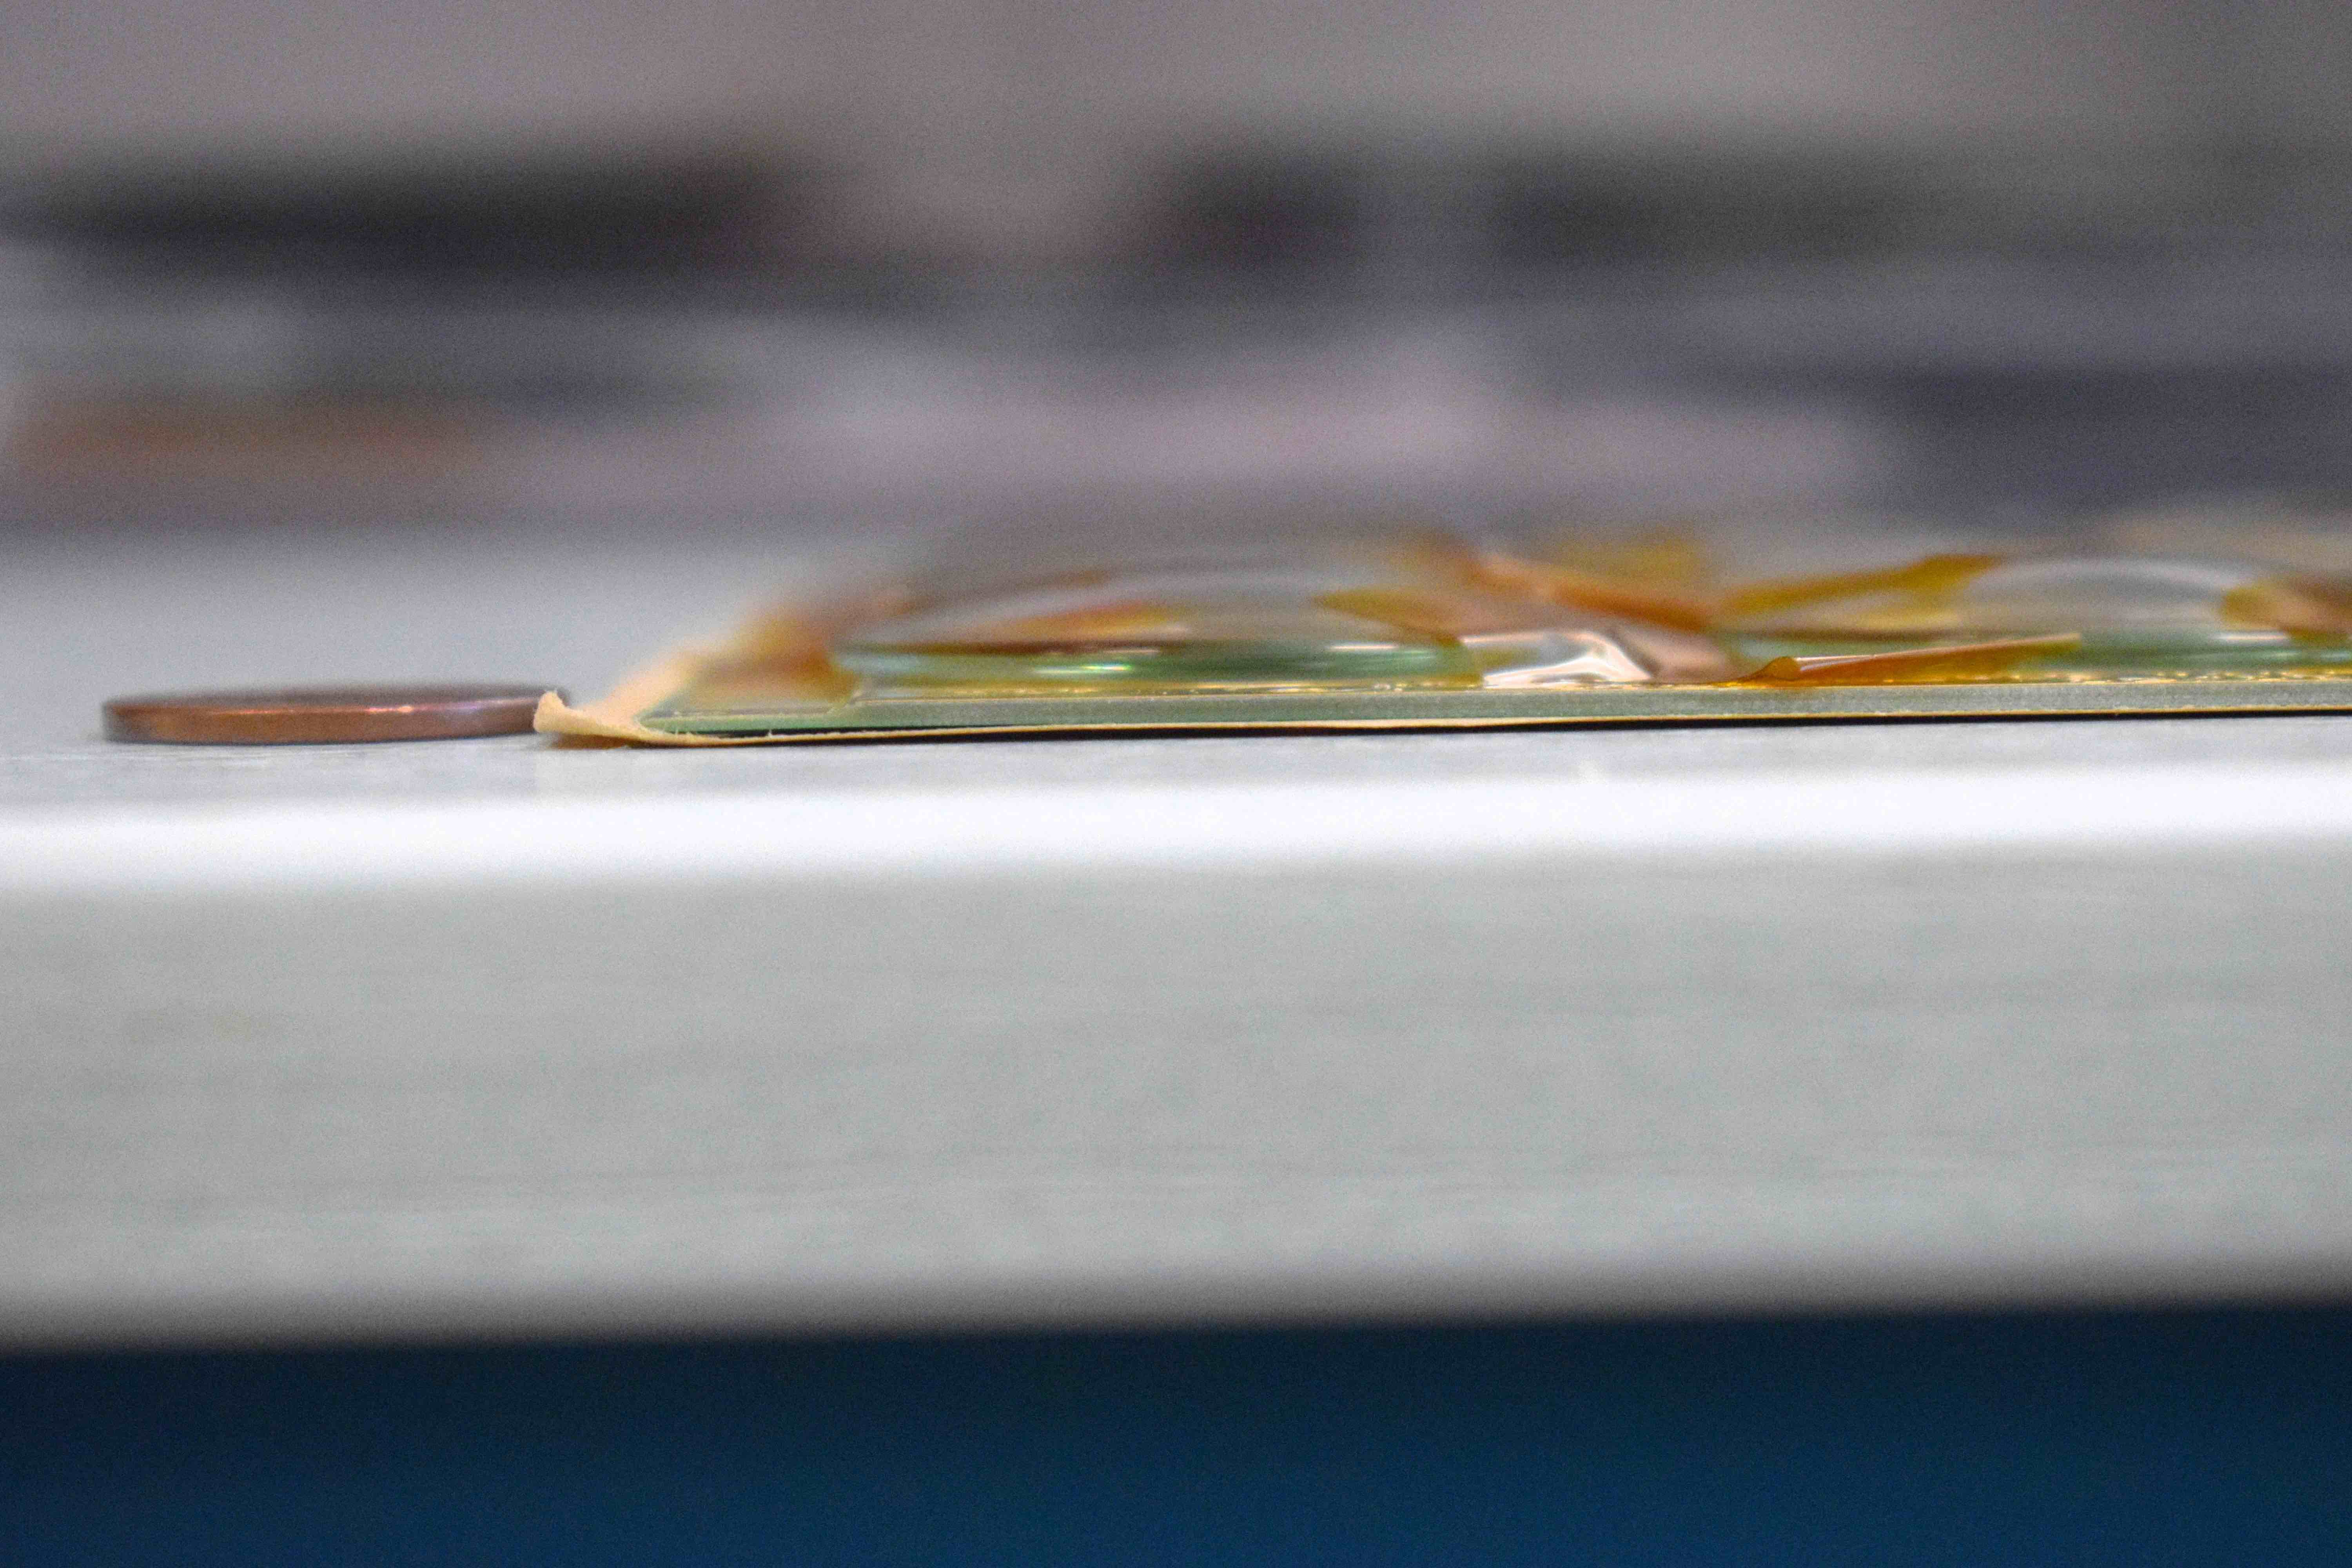
\includegraphics[width=0.38\hsize]{Detector/fig/siwecal-cob-side-red.jpg}
\caption{(Left) COB version of an ASU connected to a slab interface board. (Right) Zoom onto the edge of a COB ASU indicating its thickness.}
\label{fig:det:SiWECAL_cob}
\end{figure}



 The silicon technology developed for ILD has been adopted as the baseline for the electromagnetic end-cap section of the CMS High Granularity Calorimeter (HGCAL) upgrade~\cite{Collaboration:2293646}.
 The HGCAL layout is based on hexagonal readout modules with a technology similar to the ILD one. It incorporates a new version of the SKIROC ASIC with a sub-ns timing functionality which may also be of interest for the ILD detector.
 A HGCAL prototype of 27 layers has been successfully tested by CMS in a combined beam test at CERN with the AHCAL ILD prototype (next section). The full HGCAL represents a 10\% prototype of the ILD SiECAL w.r.t.\,the silicon diodes surface.
 Despite many differences between the ILD and CMS designs, the HGCAL construction will be a strong asset to validate the large scale assembly and fabrication processes for ILD.


 

%\textit{Sc-ECAL results from new detector unit in construction.}

\subsubsection{Scintillator option (ScECAL)}

Similar to the silicon option, the scintillator option of the electromagnetic calorimeter,
after the validation of the concept using the physics prototype,
has focused its R\&D towards a technological prototype 
with fully integrated detection layers. 
The design of the detection layer is based on an integrated readout board, 
called ECAL base unit (EBU), of $18\times18\,\mathrm{cm}^2$ 
with four SPIROC ASICs developed by OMEGA group\cite{ild:bib:spiroc} on which 144 scintillator strips 
($5\times45\times2\,\mathrm{mm^3}$ each) coupled to SiPMs are mounted.

Notable progress has recently been made on the SiPMs for the ScECAL. 
MPPCs with a smaller pixel pitch of 10 or $15\,\mu\mathrm{m}$ have been developed, which can provide a large dynamic range as required 
for the ScECAL\cite{ild:bib:hdmppc}. 
Further improvements have been made for the most recent small-pixel MPPCs, 
including reduced optical cross-talk by a trench structure between pixels, 
lower dark noise and higher photon detection efficiency. These have been confirmed by the prototype tests.

In the previous prototype studies, the SiPM was attached to the side edge 
of the strip. 
New designs of the SiPM readout at the bottom side of the strip 
are being developed for more uniform response and a better compatibility 
with future large-scale production.
Especially a recently proposed design based on a strip 
with a dimple directly coupled to a surface-mounted SiPM on the PCB, similarly to the SiPM-on-tile technology of the AHCAL (see next section),
shows a promising performance with a reasonably high light yield and a uniform response 
over the strip length (Figure~\ref{fig:det:ScWECAL_strip}).
Another design of the SiPM readout is also being studied, where the strip 
is readout by two SiPMs set in coincidence, which reduces random noise and hence improves the signal to noise ratio. For this design a twice longer strip ($L=90\,\mathrm{mm}$) is expected to be used in order
not to increase the number of SiPMs.

\begin{figure}[htb]
\centering
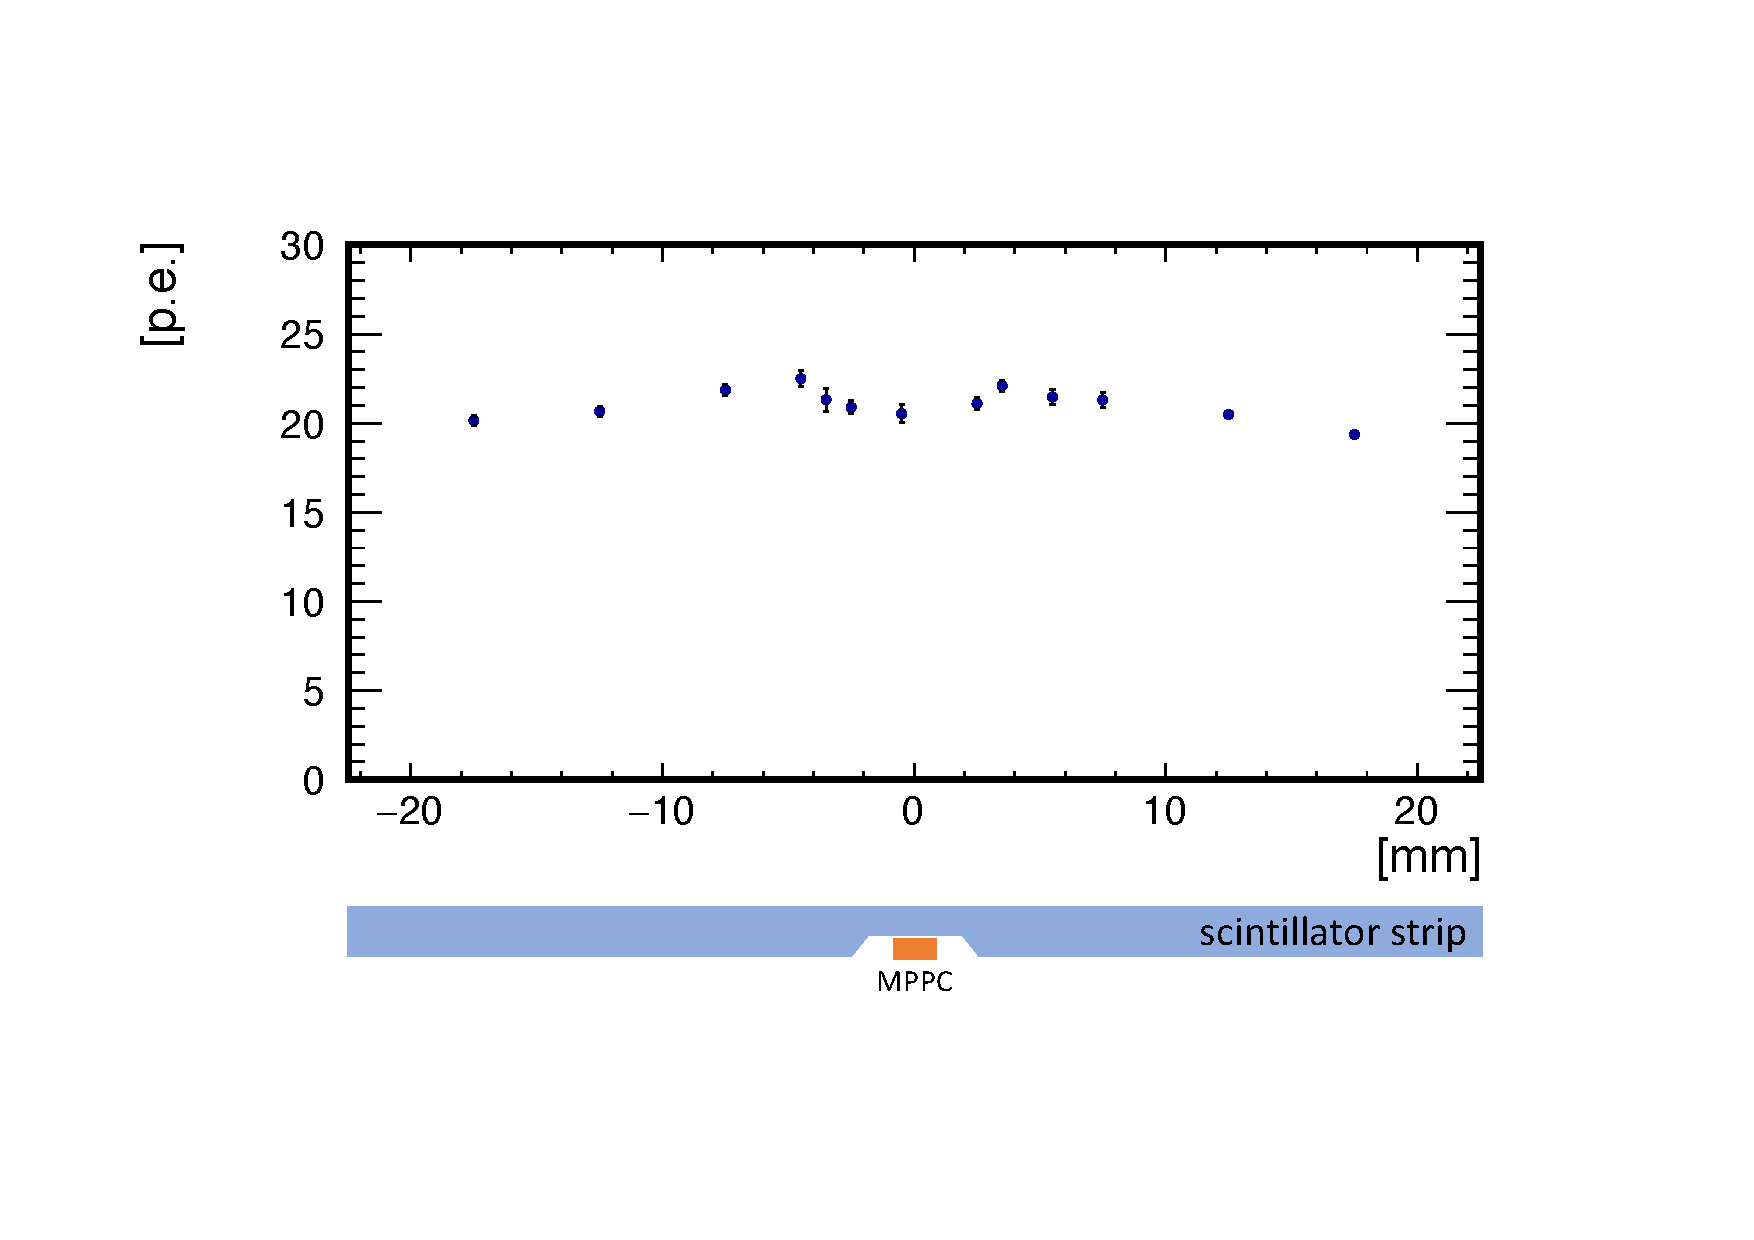
\includegraphics[width=0.7\hsize]{Detector/fig/ScWECAL_strip.pdf}
\caption{Position dependence of the light yield for the scintillator 
strip with a dimple directly coupled to a SiPM on PCB}
\label{fig:det:ScWECAL_strip}
\end{figure}


Low cost and high light yield plastic scintillator materials are also being developed 
for the ScECAL.
The development focuses on the polystyrene-based scintillator 
produced by the injection moulding method, which is suitable 
for large-scale production. 
A reasonably high light yield of 65--70\% of that of 
the commercial PVT-based scintillator, has been achieved 
by optimizing the production parameters. 

Detection layer prototypes have been developed 
with the small pixel MPPCs ($15\,\mu\mathrm{m}$ pixel pitch) 
as shown in Figure~\ref{fig:det:ScWECAL_prototype} left.
A prototype layer was tested in positron beams of 50--800\,MeV 
at the ELPH facility of the Tohoku University.
Figure~\ref{fig:det:ScWECAL_prototype} right shows the typical charge distribution 
obtained for the positron beam, with the MIP peak well separated from the pedestal.

\begin{figure}[htb]
\centering
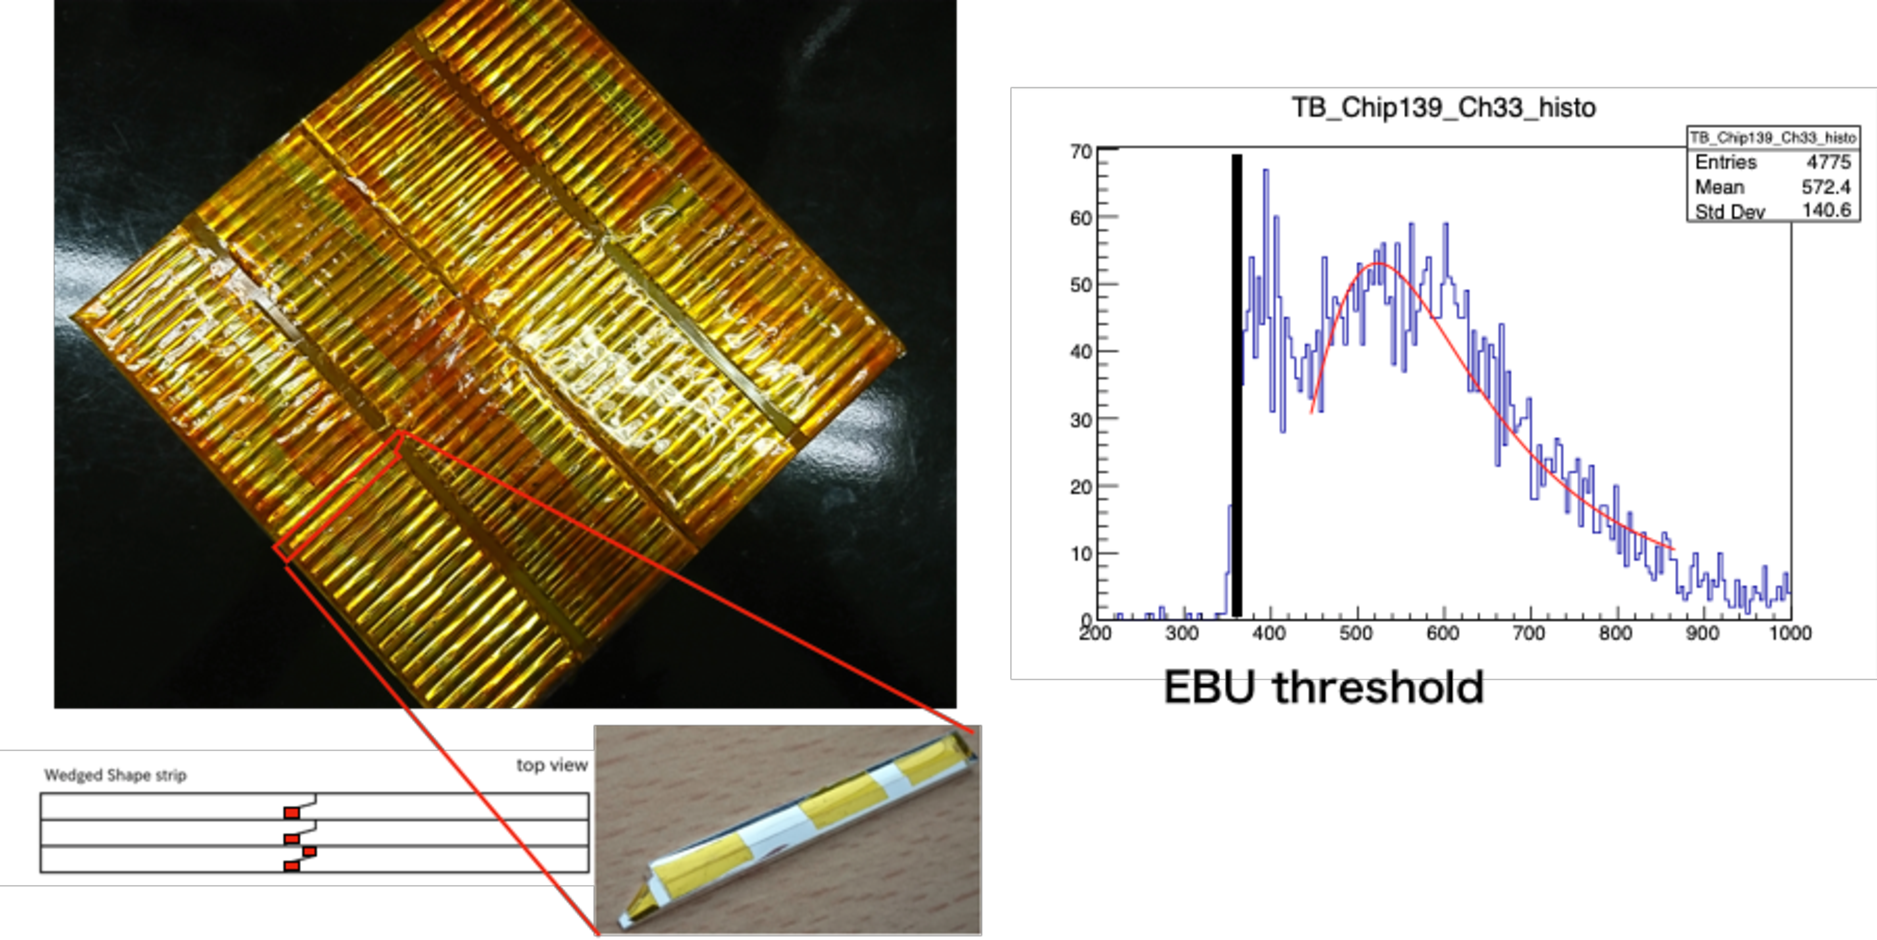
\includegraphics[width=1.0\hsize]{Detector/fig/ScWECAL_prototype.pdf}
\caption{(Left) Prototype detection layer with small pixel MPPCs  
   and (right) typical charge distribution obtained for positron beam 
where the MIP peak is well separated from the pedestal.}
\label{fig:det:ScWECAL_prototype}
\end{figure}


A fully integrated technological prototype with 30 alternating absorber and detection 
layers is planned to be constructed 
as a joint effort with the ScECAL R\&D for CEPC 
to demonstrate the performance of the ScECAL technology 
and its scalability to the full-size detector. 

